

\chapter{Search by Object Location}
\label{ch:object_location}

\emph{You see a picture in your head. Your friend was standing on the beach, and there was a little sandcastle on the left. The sea behind beautifully reflected the sun, which was setting...}

We can image, that in that particular moment we were shooting a video of the scenery. But years later, with a huge set of videos in our personal collections it may be impossible to re-watch every one of them again, to find that particular memory. Not all of us are able to visualize the memory, but those who can, we say they have a good visual memory \todo{ref}. We present a solution which can be used for searching in dataset based on such recalls of the memory.

In this chapter we elaborate solutions for known-item search task based on the visual description of the scene. The characteristics of the input are that we can recall how the objects looked (i.e. they were wearing red hoodie) and their relative location in the shot (i.e. top left corner). With those information we look the match in the database for a described scene. We encapsulate the information in input and refer to it as a \emph{collage}. It means cutting images and placing them onto empty canvas, where their placing carries also an information. We show an example of such query in the figure \ref{fig:query_collage_comparison}. On the left we can see a cat centered in the image behind the window. On the right we can see a possible visualization of such memory. The canvas is grey on which we places a window which reminded us the original one. On the center we place similarly colored cat.

\begin{figure}
\centering

\begin{subfigure}[t]{0.45\textwidth}
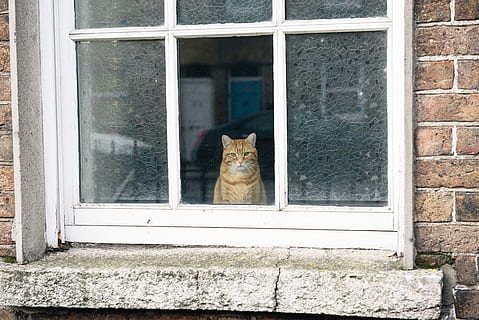
\includegraphics[width=0.9\linewidth]{img/cat_on_window} 
\caption{Query}
\label{fig:searched_scene}
\end{subfigure}
\begin{subfigure}[t]{0.45\textwidth}
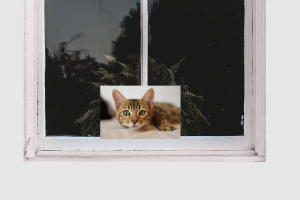
\includegraphics[width=0.9\linewidth]{img/cat_on_window_collage}
\caption{One of the possible collage description for the query}
\label{fig:collage_example}
\end{subfigure}

\caption{Example of searched scene (query) with possible visual description by a collage.}
\label{fig:query_collage_comparison}
\end{figure}

While we were describing the scene, we used words for it. But this chapter with presented solutions do not focus on the search based on the verbal description of the objects. Although, it is one of the possible alternatives to handling problem. Supporting verbal descriptions often require extensively annotated data to use to train neural networks and even though the advancements in the research area it still has a limited ability for extensively described characteristings. Our approach aims to avoid this limitations of vocabulary size semanticization fo the text.. We believe that visually we can capture more diversity. Words often either omit more specific information about the look or are hard to obtain by annotation systems, since the annotation tool may have never seen such combination before. For example, a single word for a human may represent a visually wide range of possibilities, based on clothes, age, and other attributes. We aim to avoid this bottleneck, and we proceed with the search based visual similarities.


In this chapter we utilise approaches for solving known-item search task based on \emph{collage}. Collage $C$ is a (unordered) set of $k$ pictures $C = \{\text{collage\_image}_i\} \text{for}\, i \in \{1, 2, \dots, k\} $.  Each $collage\_image_i$ contains two characteristics: image (i.e., visual description) and spatial information (location). To avoid any scaling and resolution issues, we represent location by a relative offset from the left, top, bottom and right. Therefore, all attributes of spatial information are in range $[0,1]$

This chapter will present three solutions encorporating the pretrained neural networks. To learn more about the networks head back to the chapter \todo{ref}. We start of by a short description of user-program interaction, to more understand the origin of the queries we evaluate on. The chapter invenes the ideas with their evaluation. We test different set of hyperpatameters and investigating their effect on the performance of the system. To check the dataset we work with read chapter \todo{ref}. To know more about the user interface check the documentation in the chapter \todo{ref}. 


\section{User-program interaction}

The query is a \emph{collage} of one or multiple images. Each image also includes its relative position in the canvas.

We provide a user with a canvas where she can place, move and resize the images in the \emph{collage}. Interactively, the set of results is showed (the most similar results). The user can then alternate the query for a new search, or to investigate the displayed results. The figure \ref{fig:query_collage_comparison} shows an example of the query -- the collage of two images (window and cat). 

\section{Solutions overview}

In the rest of the chapter we present different approaches to this task and we test different settings to obtain the best set of hyperparameters. In the figure \ref{fig:processing_pipeline} we can se an overview of the system. The top path is path of the database. The features are precomputed (offline) for all images in the database. We call a \emph{record} an image with it precomputed features. Each of the features may be linked also with additional information. There is one record per input image, but each record may contain multiple feature vectors describing it.

Similarly, for a given collage we extract features by using the same model as for the database extraction. We do that for each of the images in the collage. Since we only need to annotate a couple of images, this can be done online on CPU for most of the networks. In this phase, we have annotated dataset and extracted features from query images. Next, if the records contains multiple feature vectors, we may filter those to decrease the number of vectors we will compare to. We call this process \emph{Relevant Features Extraction}. As a next step, based on the features from the database and the features from the collage compute their distances, i.e., for each query image we compute the distance to each record in the database. The last step, is to merge the rankings, since each of the input images provide us with distances to records in the database. We call this step \emph{Ranking}. In the example image we can see ranking as an average of the rankings for a given record.

We tune several factors in described pipeline. Therefore, we split each step separately and we evaluate it individually. For the next sections we progressively build the pipeline, while describing the particular solutions we used. We start with feature extraction strategies and then we continue with the next steps, which are independent from features extraction.

\section{Features extraction strategies}

In the following section we present three feature extraction techniques. The feature extraction technique defines how we extract features for our dataset as well as for our queries. These obtained features will be later compared agains each other in ranking mechanism. We kick off with the baseline, where we do not use the location of the objects in the collage, only their visual representation. Then we move on onto a solution, which splits the image into regions and compare only to the regions, which relate to the object query. Our last method is experimental and it involves storing a higherdimensional feature vector. This approach aims to test a possibility for no strict cutting, rather computing based on the object location itself.

\begin{figure}[p!]
    \centering
    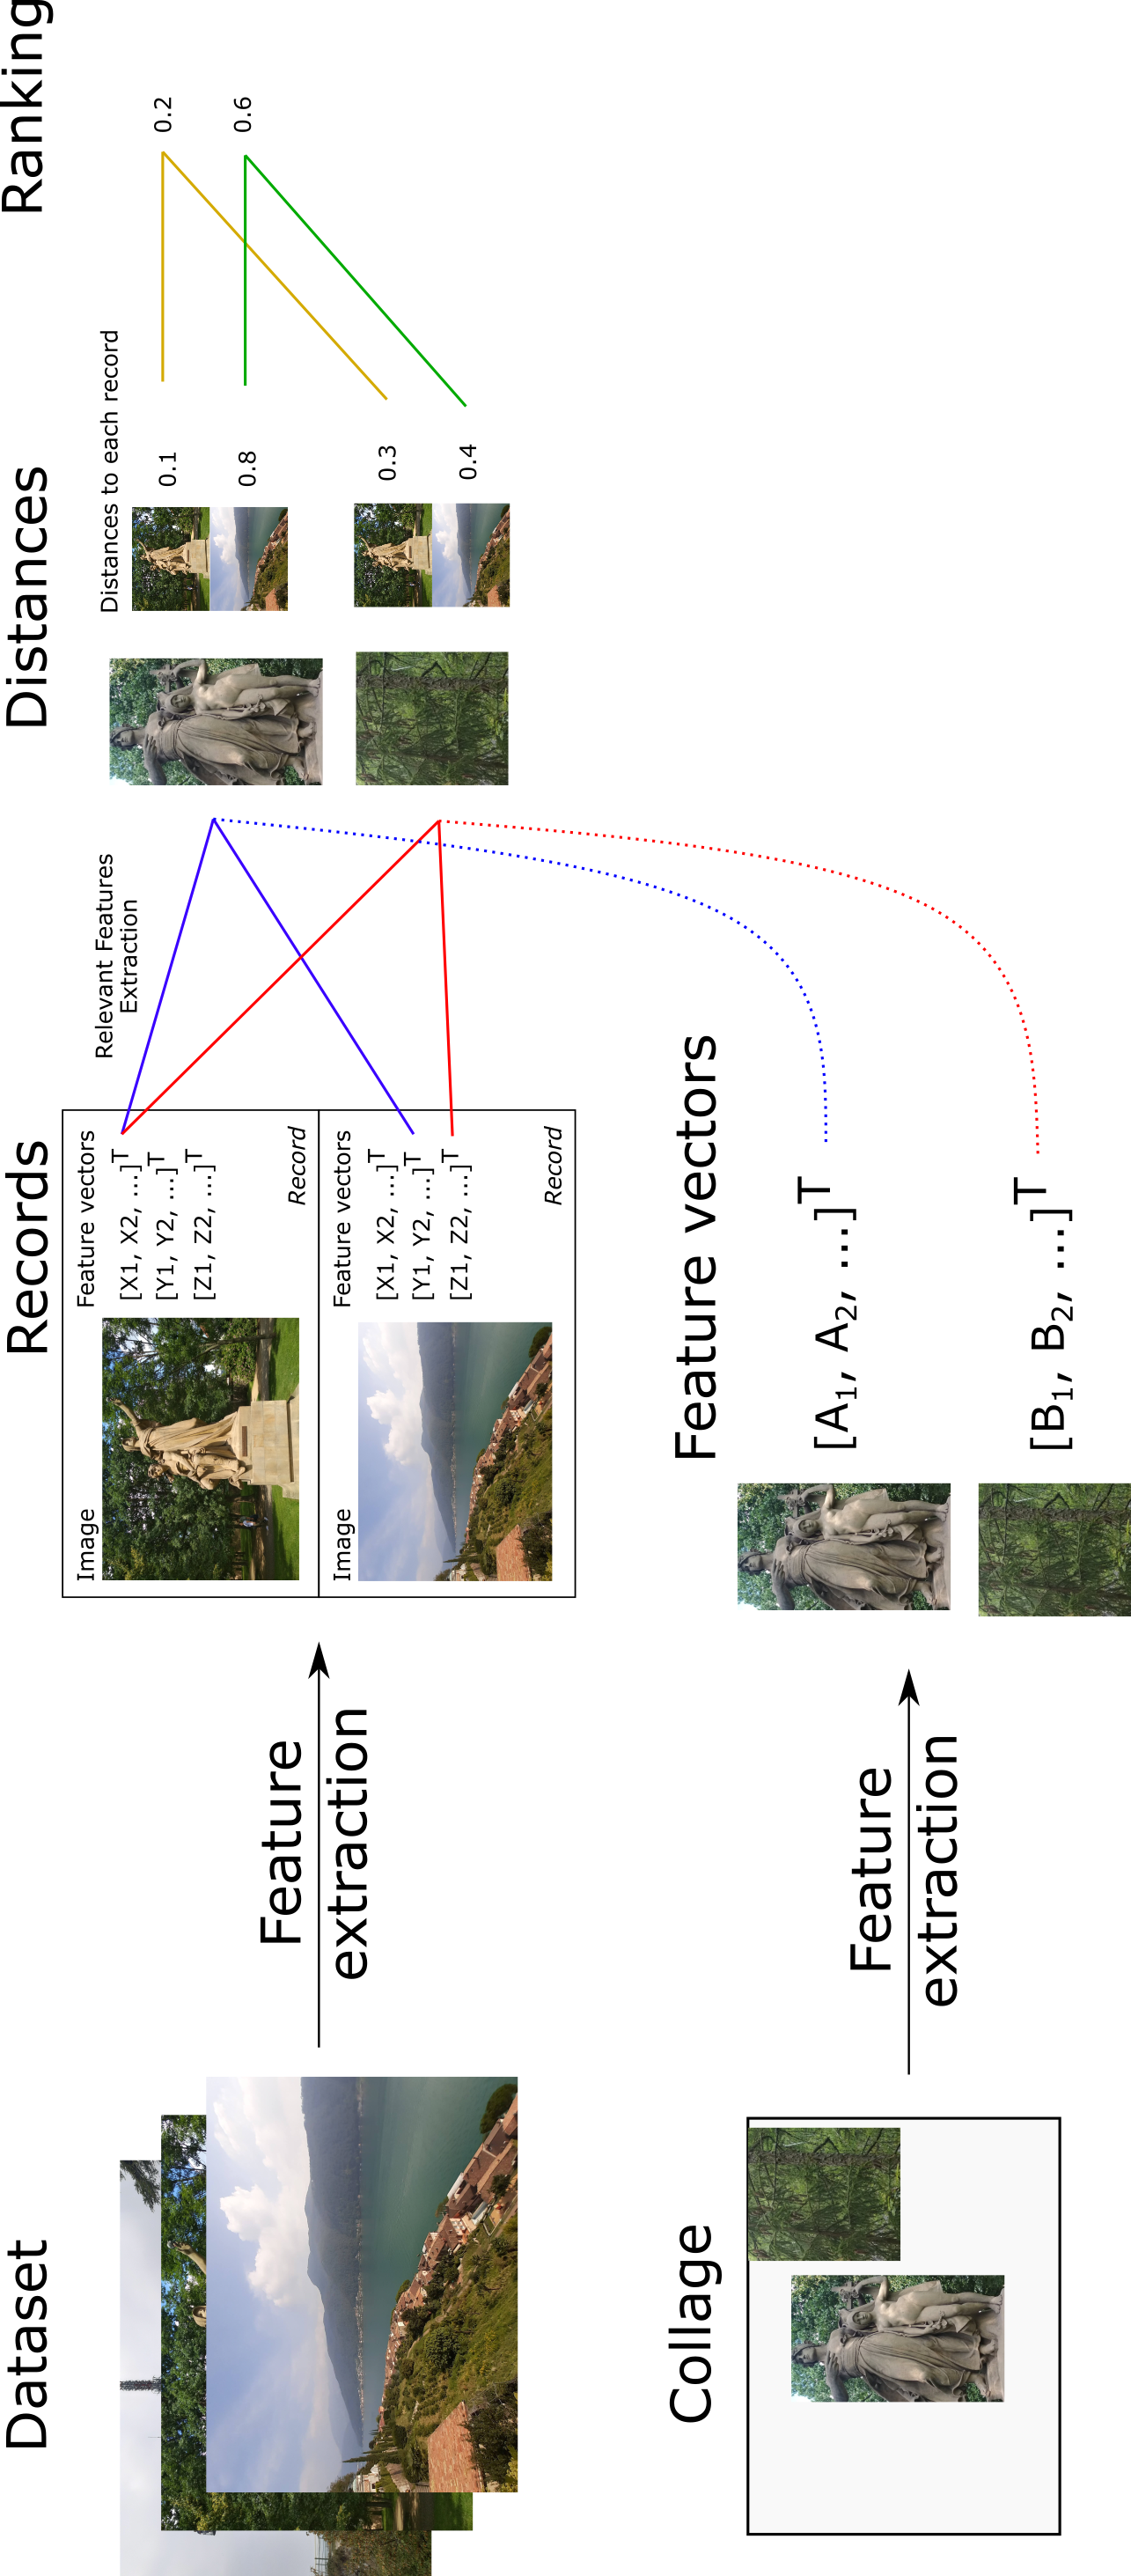
\includegraphics[scale=0.9]{img/features_pipeline_rotated.png}
    \caption{Overview of processing pipeline}
    \label{fig:processing_pipeline}
\end{figure}


\subsection{Baseline -- Image representation}

Firstly, we developed a simple approach, which ignores the information about the position of the images in the collage. We set this approach as our baseline, to see how much we improved a simple solution like this by adding more complexity. For each image in the dataset we compute one feature vector by feeding it to the pretrained convolutional neural network. The images in the dataset are rescaled (without preserving ratio) to fit the input dimensions of the network (224x224).

In the figure \ref{fig:mobilenet_whole_image} we display the performance of such approach on the annotated set of collages. We present the results on the MobileNetV2. We use MobileNetV2 due to its low computability needs and therefore offering quick annotations. It is widely used in the task, where online or near online request time is expected. We included a short description of the network in the Related Works (section \ref{}\todo{ref}).
\todo[inline]{Would be nice to add Resnet50}

\begin{figure}
\centering
\begin{boxedverbatim}
Database:
    - image: 1 feature vector (1 Dimensional)
Query:
    - query_image: 1 feature vector
    - compared to: each feature vector in the dataset
\end{boxedverbatim}
\caption{Overview of the Image representation approach}
\end{figure}

\begin{figure}
    \centering
    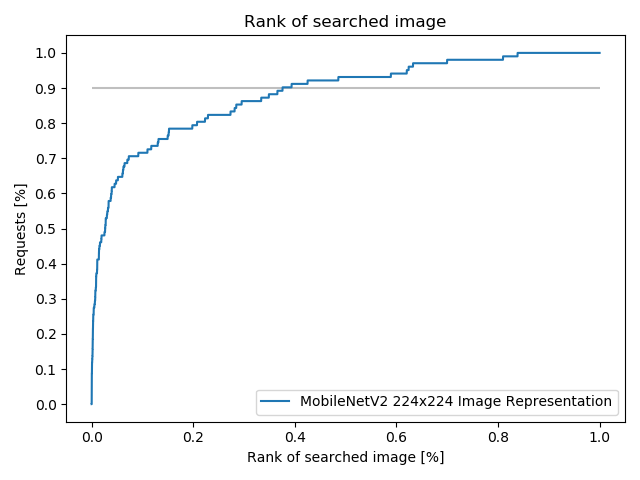
\includegraphics[width=0.8\linewidth]{img/mobilenet_whole_image.png}
    \caption{Performance of MobileNetV2 on annotated collages}
    \label{fig:mobilenet_whole_image}
\end{figure}

\subsection{Splitting an Image into Regions}

Our goal in the next presented solutions is to use also the information about objects' location. Our dataset contain many different images, with objects in different positions. Although, as we have seen in the previous section, comparison to the whole image worked well. Here we propose to include higher granularity and to split the image into multiple regions. That way we can compare the query images only to the region which is interesting (for example, if the tree is placed in bottom right corner, we would compare only to the region from bottom right corner). If we cut each image to the same regions, we will be also able to speed up the processing.

We define a cutting into a regions. Each record contain one image, which is visually divided into  $N \times M$ regions. Then for each region we compute a feature vector via pretrained model. When the query comes, we will compare the query feature vector only to the regions from the record, which overlap.

\begin{figure}
\centering
\begin{boxedverbatim}
Database:
    - image:
        - Multiple regions:
            - region coordinates
            - feature vector (1 Dimensional)
Query:


    - query_images: features vectors from M
    - compared to: only to related crops from each image
\end{boxedverbatim}
\caption{Overview of the Regions' approach}
\end{figure}



\subsubsection{Regions Shape}

In order to use transfer learning for common CNN and to avoid additional skewing in resizing, we limit to the regions only to the shape of squares. Since this input size of the square is one of the parameters, we aim to use the size of the squares the same as the size of the input of the network. This helps us to avoid unnecessary scaling which may be introduced when the length of the side of the square does not match with the input for the network.

A second limitation we create is for the regions to fully cover the record image. Since we now know we need square regions which cover a full image, there might be no way to cut image into the regions without any overlapping. Therefore, we create enough regions to fully cover the image and we split the excess between the regions. This excess is evenly distributed over the regions, creating equal overlaps. We split based on the predefined number of regions, since the number of regions results in the multiplicative coefficient for the complexity.

Allowing overlaps plays another role in this solution. With the rigid frame without overlapping, it could happen, that they would split an object into two parts. With overlaps, we know that some part is shared between both regions.

Our fixed parameters are input shape width $s$ and the number of regions we want to use $N \times M$ and image size $h, w$. We solve the task of choosing regions splits for one axis, the second is done equivalently. We know, that the last region has to end with the edge of the image. Therefore the starting coordinate of the last region is $h - s$. We then split the remaining "space" over axis over $N-1$ regions equally. We call this distance $step$, since it says the distance between the regions. The starting coordinate $r_i$ of the $i$-th region in a given axis is:

\begin{align*}
step = (h - s) / (n - 1) \\
r_i = {i \, step\,\text{for}\,i \in \{1, 2, \dots, N\}}
\end{align*}

With the condition on full coverage of the image (i.e. \(s N >= \text{h}\), and for $M$ respectively) we obtain full coverage of the image by the regions. Overlaps are evenly distributed over both axis. Although, with a bigger sized regions overlaps may occur between more than 2 regions. For example, if we split an image with width 180 into three regions with width 96 pixels, some areas of the image will be included in all three regions. This happens, when the $step <= 2 s$.

We evaluate the performance of the same network using a different number of regions. This experiment is shown in the figure \ref{fig:different_number_regions}. In the same figure we also show the effect of increasing the region width.

\todo[inline]{missing based on different size, since it was not preprocessed}
\begin{figure}
\centering
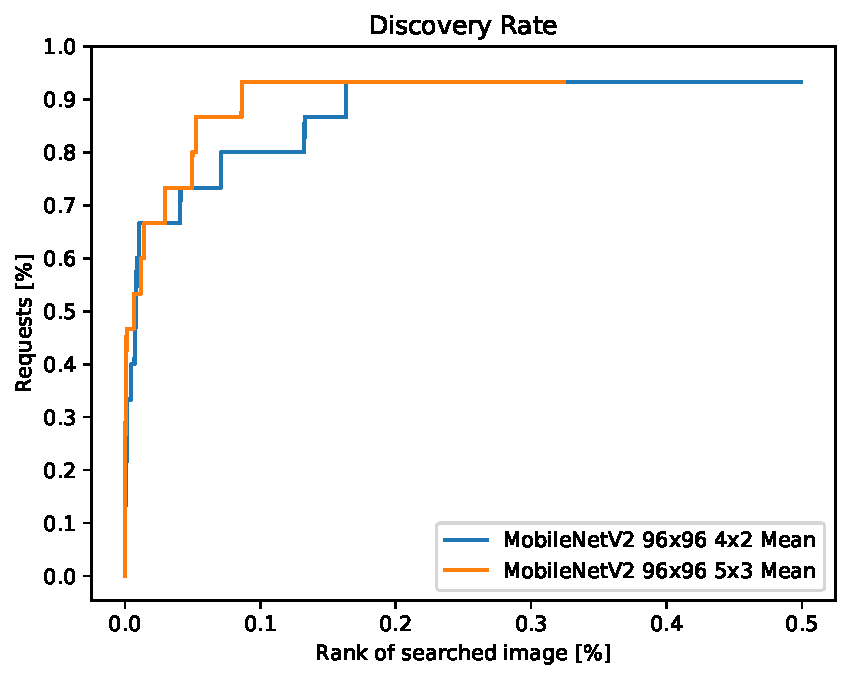
\includegraphics[width=\textwidth]{graphs/78f2a977489ac08dddac6f53446b388292306ec95f9dcbc7ca8359fbedfed9b0}
\caption{An experiment comparing the offect of the regions size and the number of regions.}
\label{fig:different_number_regions}
\end{figure}


\subsubsection{Choice of regions}

Given one incoming query image with its position and shape we propose several methods for choice of the “targeted” regions. For each one of the fixed regions we compute %\[\text{IoU_{i,j,k}} = \text{IoU}(Ri,j; Qk) for all i, j. \]

First of the options, is to only compare the region with highest Intersection over Union, limiting to the argmax IoUijk. I.e. for each i belongs I only one region would taken into account.

Second approach is to collect all intercepted regions for the similarity. This is an exhaustive process. This may result in increased computation time, i.e. usually from 2 to 9 times slower. In case of a huge set of data without any indexing, it may increase time of a request from 1 sec up to several seconds.

Third choice is to limit the number of targeted regions to a certain number. This offers us an advantage of fuller coverage and possibility for better match in neighbouring region, on the other hand provides an upper bound for the computational time required per request. 

Visualisation of chosing different number of crops can be seen in figure \ref{fig:fish_with_grid}. A comparison of the performance dependend on different number of chosen crops is shown in figure \ref{fig:crop_limitation}.

\begin{figure}
\centering
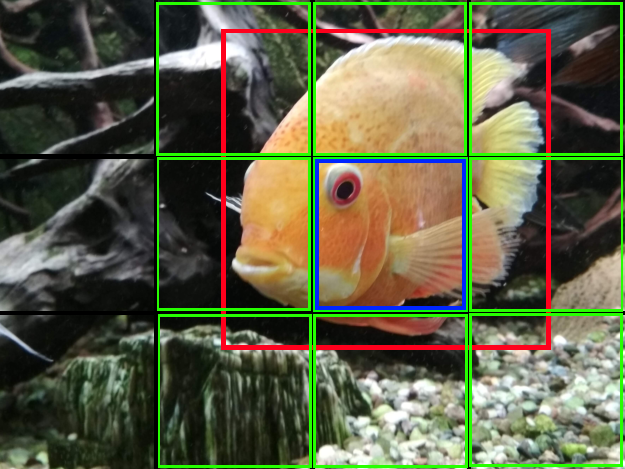
\includegraphics[width=0.6\textwidth]{img/fish_grid_regions}
\caption{Example of choosing the corresponding regions. Red: query position; Green: all intercepted regions; Blue: region with highest IoU.}
\label{fig:fish_with_grid}
\end{figure}


\begin{figure}
\centering
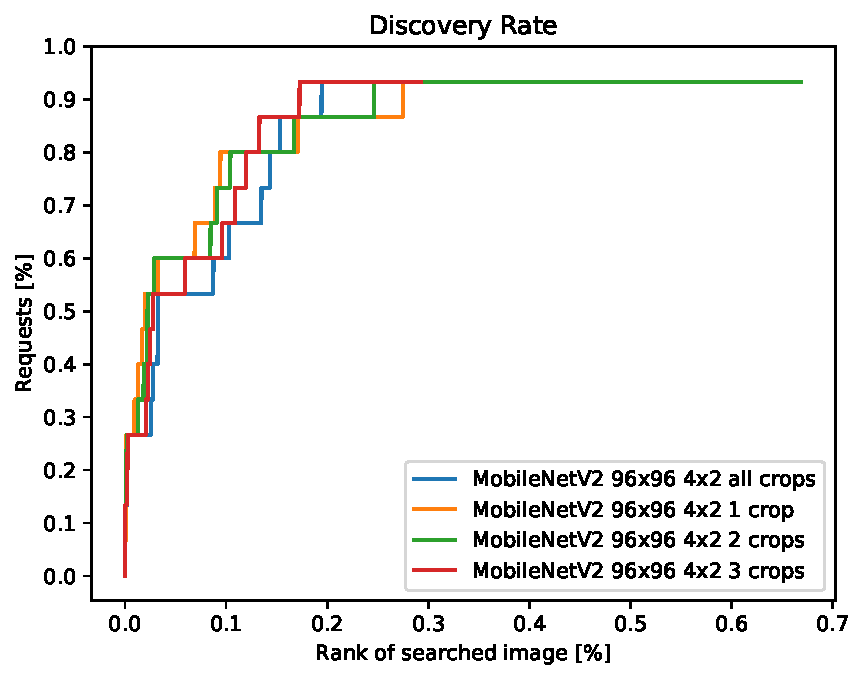
\includegraphics[width=\textwidth]{graphs/c2cf4e147040018e6cfc46043bb59de4f5f3e83441c1e1024af0b7bab644a994}
\caption{Performance of the system based on different number of chosen crops}
\label{fig:crop_limitation}
\end{figure}


\subsection{Using more information from antepenultimate layers from CNN}

The previously mentioned approach has a shortcoming. It is not able to grasp the arbitrary position of the object, rather it has limitations to previously fixed regions. This may lead to decreased performance for the objects, which cover a bigger part of the scene, i.e. in the previous case, it may overlap over multiple regions. This brings not only computational disadvantages but also reduces the amount of information which are used when compared to the query.

We propose an approach, where an antepenultimate layer of common CNN's may be used. Common CNNs are built out of several building blocks, i.e. convolution layers intervened by pooling (TODO image). This approach proved its ability for image recognition and many other related tasks (TODO add source). Many of the current state-of-the-art models use the pooling layer before fully connected layer for categorization.

We aim to leverage this antepenultimate layer, which contains not only visual features but also spatial information.

\begin{figure}
\centering
\begin{boxedverbatim}
Database:
    - image:
        - feature vector (3 Dimensional):
    - model M
Query:
    - query_images: features vectors from M, then average pool)
    - compared to: average pool over selected region for item 
                   in the database
\end{boxedverbatim}
\caption{Overview of the Spatial approach}
\end{figure}


\subsubsection{Choosing region of interest in the layer}

Layers before pooling on which we focus are 3 dimensional. First two dimensions contain spatial information, which is propagated from the previous layers. The third dimension contains visual information.

In order to obtain only a part of this layer we are interested in (i.e. our query was placed in that specific region) we need to take only a subset over first two dimensions. For a query defined by Qi = (y, x, h, w) and layer Li with first two dimensions H, W we consider a Li[y * H, x*W, (y+h) * H, (x + w) * W]. 

It is important to notice, that these layers use to have significantly lower height and width, compared to the input of the network. For example, before-last-pooling layer of Resnet50V2 has dimensions (7,7,2048). Therefore, we round our subset to nearest whole number and in case of no intersection we maintain at least intersection of size 1x1.

After this choice of the region of interest, we continue with the pooling layer in order to obtain one feature vector.

In comparison with the previous Splitting in regions approach, we see an enhanced ability to grasp more variability in object position. Especially, in queries which overlap most of the regions. On the contrary, this approach may require more memory, as for comparison for Resnet50V2 with 12 regions we needed to work only with 12 feature vectors. With the before-last-pooling layer we need for Resnet50V2 to work with 49 feature vectors. This may not be limitation with smaller feature vectors, but may come as a practical limitation based on the size of the dataset and computability power available.


\section{Ranking}
In the previous sections, we talked about the obtaining feature vector for the items in the database of the regions we are interested in. In this section, we take a closer look on further processing these obtained feature vectors.

Assuming we have an image for the query, we use the same model to compute the feature vector as was used to precompute the features for the database. Based on that we define a distance D, as the distance between the feature vector of the query and feature vector of the item in the database. This comparison to each database item gives us the distance between each item in the database and our query image.

Based on these distances we order the results, starting from the lowest to the highest distance. This distance acts as an inverse for the similarity. Similar to the results are, lower is the distance.

We use 3 main distance metrics:
Cosine Distance
Euclidean L2 distance
Euclidean L1 distance

\section{Multiple objects in the scene}

So far we talked only about handling queries consisting of one searched object. This limitation is very strict and therefore we experiment with multiple approaches to index the database based on multiple objects in the scene.

Firstly we make an assumption, that all query images have the same importance and are expected to be with the same level of relevance. Therefore we approach this problem as a set of query images, rather than as an ordered list.

We work further only with already precomputed rankings with corresponding distances for each image/part of the image. We propose several ways to merge the rankings.

We define ranking $R$ as a set of distances between the query image $q$ and database item $i$. We look for a function $r: R^n \rightarrow R$, which merges multiple rankings into one final ranking. Our goal is to minimize rank for each of the queries in the test items.

We tested several functions for this role and to compare a function that does not take into account the distances with different functions over the distances. A comparison for MobileNetV2 can be seen in figure \ref{fig:ranking_funcs}.

\begin{figure}
\centering
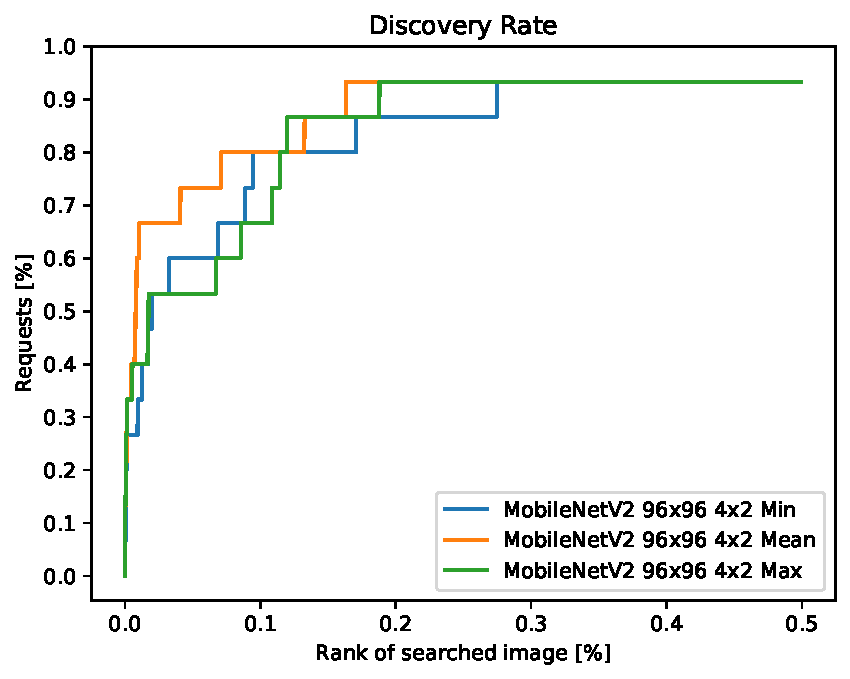
\includegraphics[width=\textwidth]{graphs/362cb9a687ce05c7732f973defca88fb8c5c393f5992066521343314698c9de7}
\caption{Performance of the system based on different fusion method}
\label{fig:ranking_funcs}
\end{figure}

\section{Padding}

Our input images provided by a user do not have to be a square images. Although, we need to prepropress these to obey the input shape of the feature extraction model we use. These models use usually square shaped input. In our case, we compare the performance of the solution based on three different approaches on input reshaping. We compare padding the input with black or white and our third option is rescaling the images. Rescaling is done in the manner, where distortion occurs for non square images, i.e, a tree becomes shorter and wider, and the car becomes narrower and taller. The results are available in the figure \ref{fig:TODO}

\section{Dimensionality reduction}

In the previous sections we evaluated several hyperparameters of the system to achieve the best performance. In this section we take a look in reducing the dimensionality of the extracted features. The extracted features from the neural networks with removed last fully connected layer are often high dimenisonality data (for MobileNetV2 its 1024 features, for Resnet50 it is 2048 features). Even though we were able to test the hyperparameters without introducing another factor -- dimensionality reduction -- we want to test also if such reduction can have also positive effects.

\todo[inline]{Mozno viac popisat PCA?}

We perform Principal Component Analysis on the extracted features. We evaluate the effects of the PCA given different number of extracted components. This helps us to significantly reduce the size of the dataset used and therefore offers us a solution with good scalability.

